\documentclass[11pt]{article}

%defines page size and margins
\usepackage{geometry}
\geometry{
  letterpaper,
  left=1in,
  right=1in,
  top=1in,
  bottom=1in,
}

%Sets spacing for entire document
\usepackage{setspace}
\singlespacing

%Package for reducing space in between list items
\usepackage{enumitem}

%Links
\usepackage{hyperref}

%Math symbols
\usepackage{gensymb}

%For floating images
\usepackage{caption}
\usepackage{float}

%better tables
\usepackage{multirow}
\usepackage{array}

\usepackage{longtable}

%Used for adjusting images
\usepackage[export]{adjustbox}

%Image path
\usepackage{graphicx}
\usepackage{animate}

\begin{document}

{\Large\noindent Jack Gregory, Brett Levenson, Andy Poulos, Rishabh Shah, John Stefan

\noindent November 21, 2017

\noindent Lab 4 \\}

\section*{Exercise One}
\begin{figure}[H]
	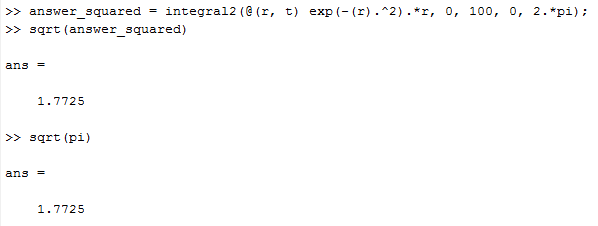
\includegraphics[width=\textwidth]{One.PNG}
	\caption*{Exercise one}
\end{figure}

\section*{Exercise Two}
\begin{figure}[H]
	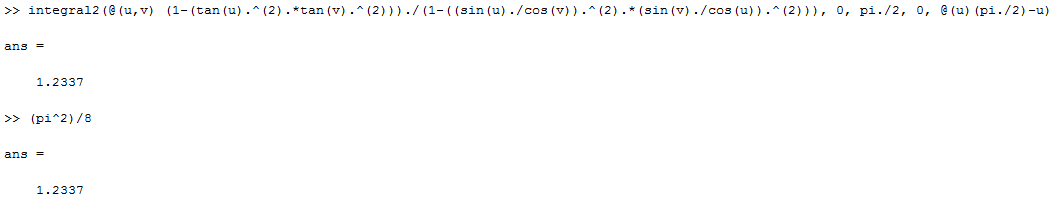
\includegraphics[width=\textwidth]{Two.PNG}
	\caption*{Exercise two}
\end{figure}

\section*{Exercise Three}


\section*{Exercise Four}
\begin{figure}[H]
	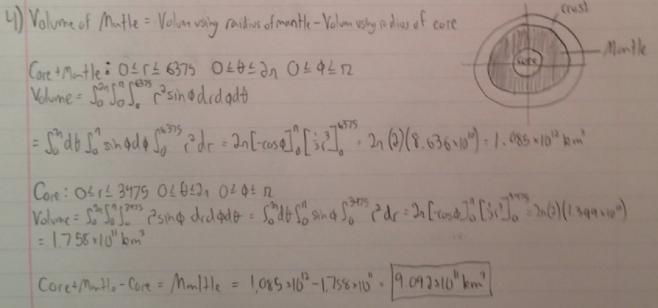
\includegraphics[width=\textwidth]{Four_Hand}
	\caption{Hand calculation for exercise four}
\end{figure}
\begin{figure}[H]
	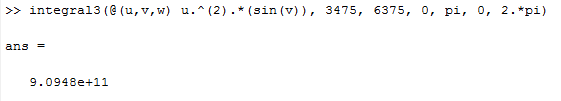
\includegraphics[width=\textwidth]{Four_Mat.PNG}
	\caption{Matlab calculation for exercise four}
\end{figure}

\section*{Exercise Five}
\begin{figure}[H]
	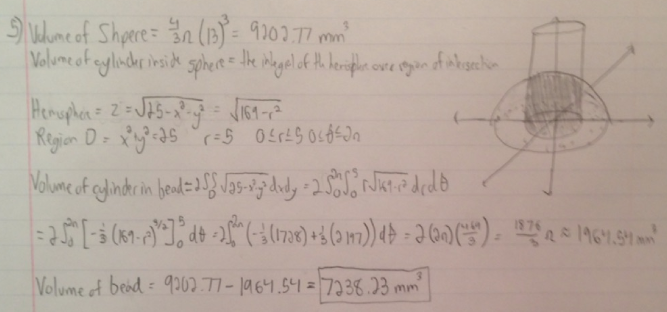
\includegraphics[width=\textwidth]{Five_Hand}
	\caption{Hand calculation for exercise five}
\end{figure}
\begin{figure}[H]
	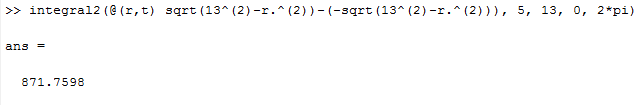
\includegraphics[width=\textwidth]{Five_Mat.PNG}
	\caption{Matlab calculation for exercise five}
\end{figure}
\end{document}